% !TeX spellcheck = en_US

\chapter{Concept and Architecture}\label{chap:conarch}
In this chapter, the concept and the architecture of the framework, which can satisfy the requirements will be described and substantiated.
Solutions to some additional problems will be presented. 
\section{Concept}
In this section, the main concept of this work will be described.
The general structure of the framework is represented in the block diagram \ref{fig:gen}. 
In the section~\ref{subs:analyse}, it will be found out how to determine during the preprocessing stage which Node Templates uses the given artifact.
Then a functionality of language modules and package manager modules is described.
In the section~\ref{subs:repres}, it will be explained how to create a new node for a TOSCA topology. 
After that, a problem of the determining the architecture of the final platform will be explained and a solution described.
In additional, it will be described, how the results can be validated.
% !TeX spellcheck = en_US

\begin{figure}
	\centering
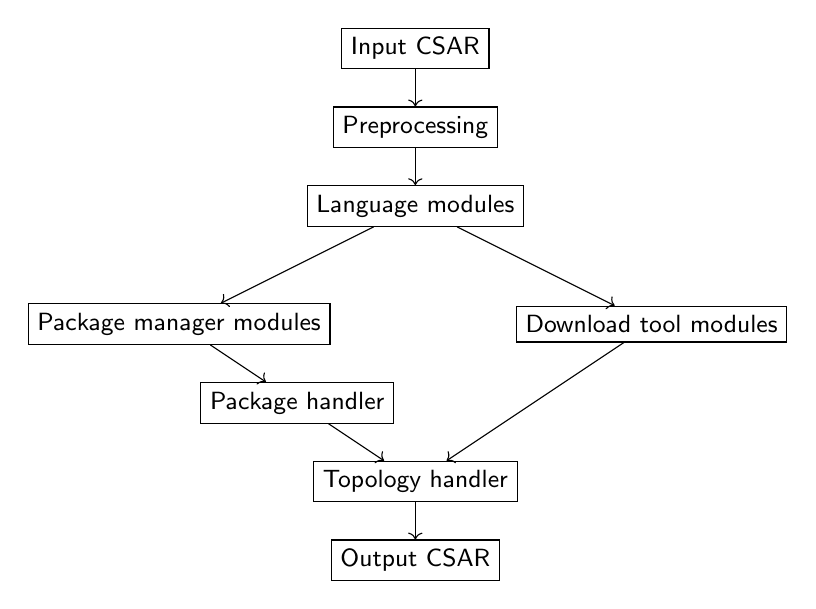
\begin{tikzpicture}
\node[draw] (in) at (0,1.5) {Input CSAR};
\node[draw] (pp) at (0,+0.5) {Preprocessing};
\node[draw] (lm) at (0,-0.5) {Language modules};
\node[draw] (pmm) at (-3,-2) {Package manager modules};
\node[draw] (dtm) at (+3,-2) {Download tool modules};
\node[draw] (ph) at (-1.5,-3) {Package handler};
\node[draw] (th) at (0,-4) {Topology handler};
\node[draw] (out) at (0,-5) {Output CSAR};
\draw [->] (in) -- (pp);
\draw [->] (pp) -- (lm);
\draw [->] (lm) -- (pmm);
\draw [->] (lm) -- (dtm);
\draw [->] (pmm) -- (ph);
\draw [->] (dtm) -- (th);
\draw [->] (ph) -- (th);
\draw [->] (th) -- (out);
\end{tikzpicture} 
\caption{The general description of the software's work flow} 	\label{fig:gen}
\end{figure}


\subsection{Analysis existing TOSCA-Topology}\label{subs:analyse}
To properly update the \gls{tosca} topology, it is necessary to add references from the nodes where external references were to newly created nodes, which resolve the external references. 
According to the TOSCA standard, only references between Node Templates in the same Service Template can be created.  
That means that each Node Template, which uses artifacts with external references must be found.
Furthermore, Service Template where these Node Templates are instantiated must be found to create there a Node Template for the new nodes and reference them to the Node Templates with external references.
The Pointers to Artifacts are contained by Artifact Templates, which are used by Node Type Implementations.
By composing all the information a simple references chain can be built:\\
$Artifact$ $\rightarrow$ $Artifact$~$Template$ $\rightarrow$ $Node$~$Type$~$Implementation$ $\rightarrow$ $Node$~$Type$ $\rightarrow$ $Node$~$Template$ $\rightarrow$ $Service$~$Template$\\
Now consider the references in more detail. 
\begin{itemize}
	\item $Artifact$ $\rightarrow$ $Artifact$ $Template$\\
	An Artifact can be referenced by several Artifact Templates. (Despite the fact that this is a bad practice.)
	\item  $Artifact$ $Template$ $\rightarrow$ $Node$ $Type$ $Implementation$ \\
	The same way an Artifact Template can be used by several Node Type Implementations.
	\item $Node$ $Type$ $Implementation$ $\rightarrow$ $Node$ $Type$ \\
	A Node Type Implementation can describe an implementation of only one Node Type.
	\item  $Node$ $Type$ $\rightarrow$ $Node$ $Template$\\
	Each Node Type can have any number of Node Templates.
	\item  $Node$ $Template$ $\rightarrow$ $Service$ $Template$\\
	But each Node Template is instantiated only once.
\end{itemize}
Thus structure can be described by a tree with an Artifact as the root, and Service Templates as leaves (The example is on figure \ref{fig:script_serv}) and will be called the internal dependencies tree.
% !TeX spellcheck = en_US
\usetikzlibrary{calc,arrows.meta,positioning}
\tikzset{
    every node/.style={font=\sffamily\small},
    main node/.style={shape=rectangle, rounded corners,
    	draw, align=center,
    	top color=white, bottom color=blue!20}
}

\begin{figure}
	\centering
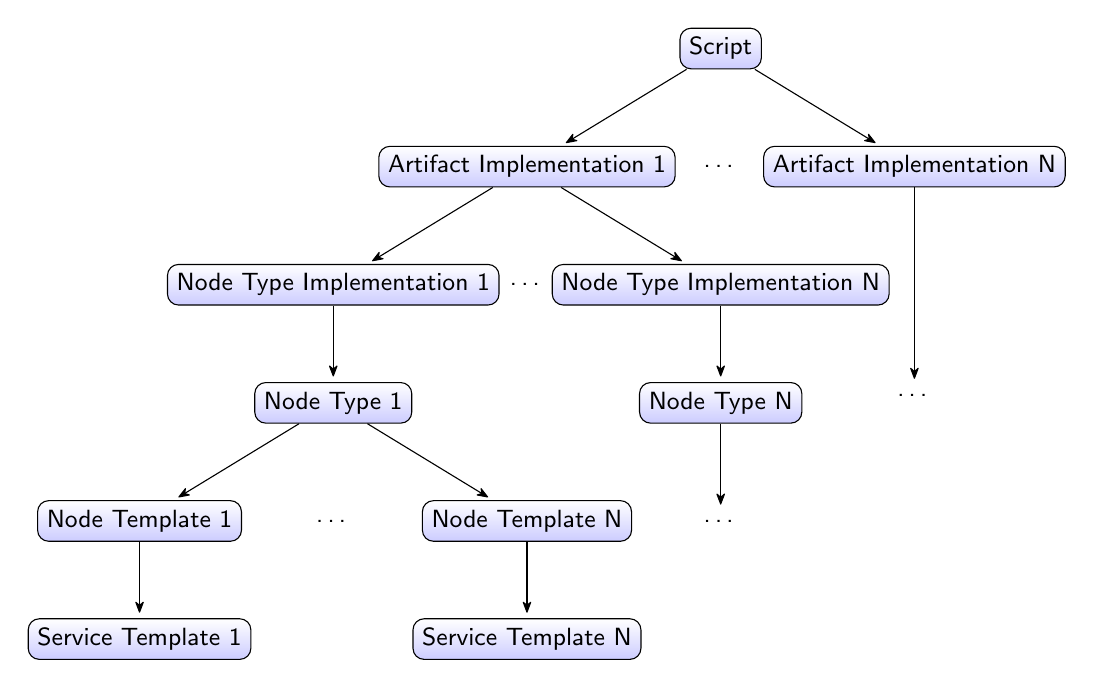
\begin{tikzpicture}[sibling distance=14em,->,>={Stealth[round,sep]},shorten >=1pt,auto,node distance=25mm]
    \node[main node] (1) {Script}
    child { node[main node](3) {Artifact Implementation 1} 
    	child { node[main node] (6) {Node Type Implementation 1} 
    			child { node[main node] (8) {Node Type 1} 
    				child { node[main node]  (11) {Node Template 1} 
    					child { node[main node] (13) {Service Template 1}}  
    				}
    				child { node[main node]  (12) {Node Template N} 
    					child { node[main node] (14) {Service Template N}}
    				}
    			}
    	}
    	child { node[main node] (7) {Node Type Implementation N} 
    		child { node[main node] (9) {Node Type N} 
    			child { node  (10) {\ldots} }
    		}
    	}
    }
    child { node[main node] (4) {Artifact Implementation N}  
    child { node (5) [below =of 4]{\ldots}}
	};

    \node at ($(3)!.5!(4)$) {\ldots};
    \node at ($(6)!.5!(7)$) {\ldots};
    \node at ($(11)!.5!(12)$) {\ldots};
    
\end{tikzpicture} 
\caption{Example tree describing how to find Service Templates and Node Templates for a given script} 	\label{fig:script_serv}
\end{figure}
%Of course it is possible to move in opposite direction, starting from a Node and moving toward scripts, but this method brings additional complexity. 
An additional problem is in the reference between a Node Type and a Node Type Implementation.
Node Type can have several implementations, but which one will be used will be determined only during the deployment. 
The chosen solution to this problem is to use each Node Type Implementation in hope, that they will not conflict.\\
%The method presented above can uniquely determine Node Templates and Service Template for a given script.
%Of course it is not guaranteed that found Node Type Implementation will be used during deployment, but we can't do anything with this. 
The following steps can be executed during the preprocessing, to build the internal dependencies tree.
\begin{itemize}
	\item Find all Artifact Templates to build references from Artifacts to Artifact Templates.
	\item Find all Node Type Implementations. Because they contain references both to the Node Type and to the Artifact Templates, then the dependency from Artifact to Node Types can be built.
	\item Find all Service Templates and in them contained Node Templates. Each Node Template contains a reference to Node Type, what is useful for building a dependency from Artifact to Node Template.
\end{itemize} 
In this way, the required internal dependencies tree can be built (with references $Artifact$ $\rightarrow$ $Node$~$Template$ and $Artifact$ $\rightarrow$ $Service$~$Template$).

\subsection{Modules and extensibility}
Unfortunately, it is impossible to identify all types of external references, even when only one language and one package manager are used (an example in the listing \ref{alg:unreadable}).
\begin{Listing} 
	\caption{Unreadable bash script}
	\label{alg:unreadable}
\begin{lstlisting}
#!/bin/bash
set  line = abcdefgijklmnoprst
set  word1 = ${line:0:1}${line:14:1}${line:17:1} 
set  word2 = ${line:6:1}${line:4:1}${line:17:1}
$word1-$word2 install package
\end{lstlisting}
\end{Listing}
Since this work is aimed at creating of the easily expanded and supplemented tool, initially only basic usage of package managers will be considered.\\
The framework should handle different languages, each of them can support various package managers.
A language module should filter files not belonging to the language, and accepted files will be transmitted to corresponding package manager modules.
This principle can be illustrated by a figure \ref{fig:lang_pm}.
% !TeX spellcheck = en_US

% We need layers to draw the block diagram
\usetikzlibrary{calc,positioning}

% Define a few styles and constants
\tikzstyle{entry}=[draw, fill=green!20, minimum height=2.5em]
\tikzstyle{ann} = [above, text width=5em]
\tikzstyle{framework} = [entry, text width=35em, fill=red!20, 
minimum height=18em, rounded corners]
\tikzstyle{lang} = [entry, text width=9em, fill=blue!20, 
minimum height=15em, rounded corners]
\def\blockdist{2.3}
\def\edgedist{2.5}

\begin{figure}
	\centering
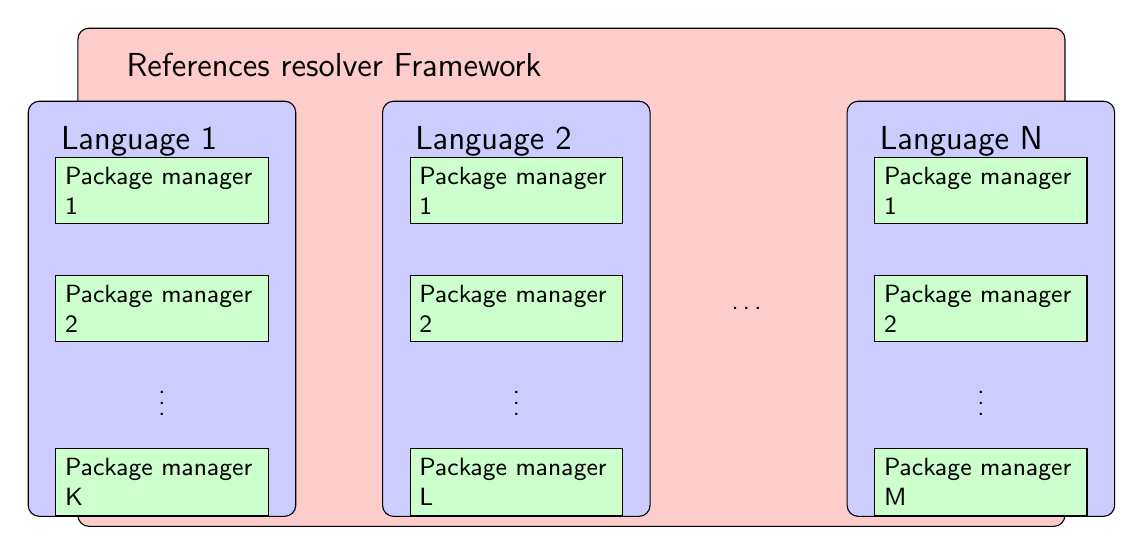
\begin{tikzpicture}
\node (rr) [framework] {};
\node [xshift=+5mm, yshift=-2mm, below right] at (rr.north west) {\large References resolver Framework };


\node (lang1) at ([xshift=-52mm,yshift=-4mm]rr) [lang] {};
\node [xshift=+3mm, yshift=-2mm, below right] at (lang1.north west) {\large Language 1 };
\node (lang2) at ([xshift=-7mm,yshift=-4mm]rr) [lang] {};
\node [xshift=+3mm, yshift=-2mm, below right] at (lang2.north west) {\large Language 2 };
\node (langn) at ([xshift=+52mm,yshift=-4mm]rr) [lang] {};
\node [xshift=+3mm, yshift=-2mm, below right] at (langn.north west) {\large Language N };
\node at ($(lang2)!.5!(langn)$) {\ldots};

\node (l1pm1) at ([yshift=+15mm]lang1) [entry] {Package manager 1};
\node (l1pm2) at ([yshift=0mm]lang1) [entry] {Package manager 2};
\node (l1pmn) at ([yshift=-22mm]lang1) [entry] {Package manager K};
\node at ($(l1pm2)!.5!(l1pmn)$) {\vdots};

\node (l2pm1) at ([yshift=+15mm]lang2) [entry] {Package manager 1};
\node (l2pm2) at ([yshift=0mm]lang2) [entry] {Package manager 2};
\node (l2pmn) at ([yshift=-22mm]lang2) [entry] {Package manager L};
\node at ($(l2pm2)!.5!(l2pmn)$) {\vdots};

\node (lnpm1) at ([yshift=+15mm]langn) [entry] {Package manager 1};
\node (lnpm2) at ([yshift=0mm]langn) [entry] {Package manager 2};
\node (lnpmn) at ([yshift=-22mm]langn) [entry] {Package manager M};
\node at ($(lnpm2)!.5!(lnpmn)$) {\vdots};


\end{tikzpicture} 
\caption{Example scheme representing several languages and package managers} 	\label{fig:lang_pm}
\end{figure}
A package manager module resolves an external reference and transmits the package name to a package handler, described in section \ref{subs:archph}.\\
The framework will contain a list of all supported language modules, and each language module will contain a list of supported package managers modules.
Ease of adding new modules to the framework will proof the correctness of the architecture.\\
At the beginning, the most popular combination will be implemented: the $bash$ language with the $apt-get$ package manager.
This simple and powerful tool allows to install, delete or update the set of packages in one line.
A line-by-line parser should be developed, which analyses scripts and finds the installation commands.
After the modules for this combination will be implemented, new language and package manager modules should be added.

\subsection{Representing downloaded packages in TOSCA-Topology} \label{subs:repres}
A package node denotes to the defined and instantiated element of \gls{tosca} topology, the purpose of which is to install the package.
The adding of new package nodes to TOSCA topology can be divided into several steps.
\begin{itemize}
	\item Add definitions for common elements, like Artifact Types or Relationship Types. 
		This can be done once at the preprocessing stage.
	\item The package node main definition will be represented by a Node Type. 
		%There will be described that this node must be installed.
	\item Artifacts (The downloaded data and the installation script) will be referenced by Artifact Templates.
	\item Node Type Implementation will combine the artifacts.
	\item Node Template will instantiate the package node in the corresponding Service Templates.
		To determine corresponding Service Template the preprocessing described in the section \nameref{subs:analyse} will be used.
	\item Reference Template will provide topology information, allowing the observer (a user or a runtime environment) to determine, for which nodes the package must be installed.
		References will be created from the Node Template needing the package to Node Template of created package nodes.
\end{itemize}
After an execution of those steps, a definition of a package node will be finished and this node can be used.
\subsection{Determining architecture of a final platform}
An another problem appears during choosing the architecture of the device where packages will be installed.
Unfortunately, it is impossible to analyze the structure of any CSAR and give an unambiguous answer to the question, on which architecture which node will be deployed.
There are many pitfalls here.\\
A single Service Template can use several physical devices with different architectures.
One Implementation Artifacts can be referred by different Node Types and Node Templates, instantiated on different platforms.
This way one simple Implementation Artifact with a bash script containing "$apt$-$get$ $install$ $python$" command can be deployed on different devices within one Service Template (for example with the arm, amd64 and i386 architectures) and will result in the loading and installation of three different packages. 
For an end user, the ability to use such a simple command is a huge advantage, but for the framework, it can greatly complicate analysis.
The following methods of architecture selection were designed.
\begin{itemize}
	\item $Deployment$ $environment$ $analysis$\\
	The script can analyze the system where it was started (for example using the "$uname$~$-a$" command) and depending on the result, it will install the package corresponding to the system's architecture.
	\item $Unified$ $architecture$\\
	The architecture will be defined by the user for a whole CSAR.
	\item $Artifact$ $specific$ $architecture$\\
	The architecture will be defined separately for each artifact.
\end{itemize}
\subsubsection*{Analysis of methods}
The $deployment$ $environment$ $analysis$, which at first sight seems to be the most reliable solution, brings many additional problems.
Packages for different platforms can differ not only by architecture but also by the version and the list of dependencies.
As a consequence, a chaos can be produced by mirroring these different packages with different versions to the \gls{tosca}-topology.
The only robust solution seems to be to create for each installed package a set of archives (one archive for one architecture), containing the entire dependency tree for the given package.
But this approach contradicts one of the main ideas of this work: the dependencies trees should be mapped to the topology.\\
The $artifact$ $specific$ $architecture$ method carries an additional complexity to the user of the framework.
It will obligate a user to analyze each artifact and decide on which architecture it will be executed. 
This can be complicated by the fact that the same artifact can be executed on different architectures.\\
The method of the $unified$ $architecture$ was chosen, as the simplest and easiest to implement.
If it will be necessary, this method can be easily expanded to the $artifact$ $specific$ $architectures$ method (By removing the user input at start, and choosing an architecture for each artifact separately.) or to $deployment$ $environment$ $analysis$ (By downloading packages for all available architectures and adding the architecture determining algorithm to the installation scripts.).

%\subsection{Extensibility}
%The framework should handle different languages, each of them can support various package managers.
%An language module should filter files not belonging to the language, accepted files will be processed 
%This principle can be illustrated by a figure \ref{fig:lang_pm}.
%% !TeX spellcheck = en_US

% We need layers to draw the block diagram
\usetikzlibrary{calc,positioning}

% Define a few styles and constants
\tikzstyle{entry}=[draw, fill=green!20, minimum height=2.5em]
\tikzstyle{ann} = [above, text width=5em]
\tikzstyle{framework} = [entry, text width=35em, fill=red!20, 
minimum height=18em, rounded corners]
\tikzstyle{lang} = [entry, text width=9em, fill=blue!20, 
minimum height=15em, rounded corners]
\def\blockdist{2.3}
\def\edgedist{2.5}

\begin{figure}
	\centering
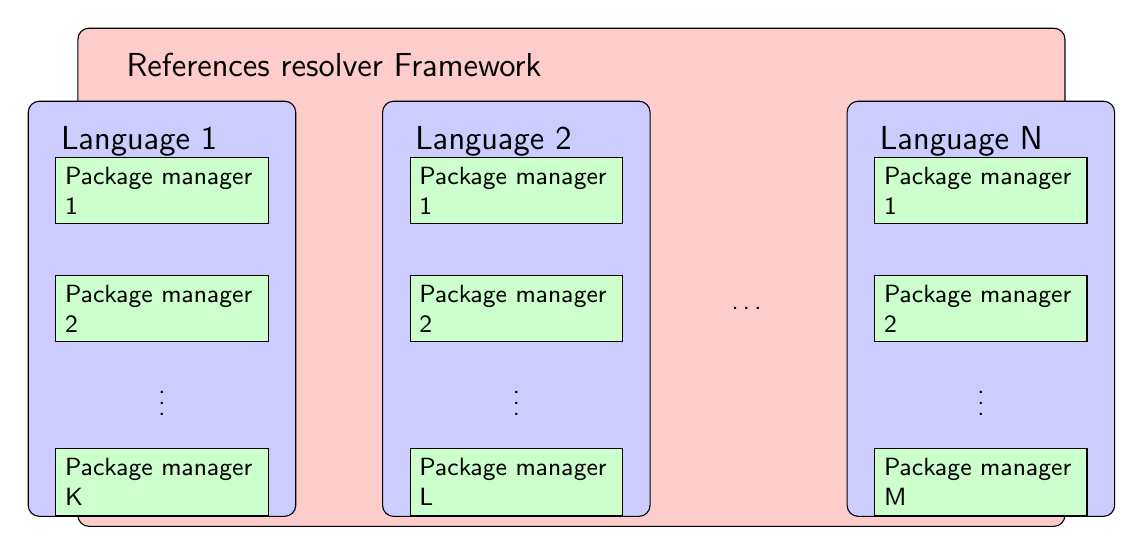
\begin{tikzpicture}
\node (rr) [framework] {};
\node [xshift=+5mm, yshift=-2mm, below right] at (rr.north west) {\large References resolver Framework };


\node (lang1) at ([xshift=-52mm,yshift=-4mm]rr) [lang] {};
\node [xshift=+3mm, yshift=-2mm, below right] at (lang1.north west) {\large Language 1 };
\node (lang2) at ([xshift=-7mm,yshift=-4mm]rr) [lang] {};
\node [xshift=+3mm, yshift=-2mm, below right] at (lang2.north west) {\large Language 2 };
\node (langn) at ([xshift=+52mm,yshift=-4mm]rr) [lang] {};
\node [xshift=+3mm, yshift=-2mm, below right] at (langn.north west) {\large Language N };
\node at ($(lang2)!.5!(langn)$) {\ldots};

\node (l1pm1) at ([yshift=+15mm]lang1) [entry] {Package manager 1};
\node (l1pm2) at ([yshift=0mm]lang1) [entry] {Package manager 2};
\node (l1pmn) at ([yshift=-22mm]lang1) [entry] {Package manager K};
\node at ($(l1pm2)!.5!(l1pmn)$) {\vdots};

\node (l2pm1) at ([yshift=+15mm]lang2) [entry] {Package manager 1};
\node (l2pm2) at ([yshift=0mm]lang2) [entry] {Package manager 2};
\node (l2pmn) at ([yshift=-22mm]lang2) [entry] {Package manager L};
\node at ($(l2pm2)!.5!(l2pmn)$) {\vdots};

\node (lnpm1) at ([yshift=+15mm]langn) [entry] {Package manager 1};
\node (lnpm2) at ([yshift=0mm]langn) [entry] {Package manager 2};
\node (lnpmn) at ([yshift=-22mm]langn) [entry] {Package manager M};
\node at ($(lnpm2)!.5!(lnpmn)$) {\vdots};


\end{tikzpicture} 
\caption{Example scheme representing several languages and package managers} 	\label{fig:lang_pm}
\end{figure}

\subsection{Result's checking}
Checking the output of the framework is an important stage in the development of the program.
It is necessary to verify both the overall validity of the output \gls{csar} and the possibility to deploy generated package nodes.
To test for overall correctness it is possible to use $winery$ tool from OpenTOSCA.
This tool for creating and editing CSAR archives is also great for visualizing the results.
Checking the deployment of the generated package nodes can be done manually by entering commands starting the implementation artifact's execution.

\section{Architecture}\label{sec:arch}
This section will present the architecture of the framework and the detailed description of its elements.
The main elements are a $CSAR$ $handler$, a $references$ $resolver$, $language$ $modules$, $package$ $manager$ $modules$, a $package$ $handler$, and a $topology$ $handler$.

\subsection{CSAR handler} \label{subs:casr_h}
The CSAR handler provides an access to a \gls{csar} and maintains it's consistency. 
It describes the processes of the adding of new files (to handle the metadata), archiving/unarchiving, and the choosing of a final platform architecture.

\subsection{References resolver} \label{subs:RR}
This is the main element, the execution of which can be divided into the three stages: $preprocessing$, $processing$, $finishing$. \\
During the $preprocessing$ stage, the CSAR will be unarchived, common files added, and internal dependencies trees generated.
Figure \ref{fig:preproc} illustrates those steps.
During the $processing$, all $language$ $modules$ will be activated, which are described in more details in the next section. \\
To finish the work all results will be packed to the output CSAR during the $finishing$ stage.
% !TeX spellcheck = en_US

\usetikzlibrary{calc,arrows.meta,positioning,arrows}
\tikzset{
    every node/.style={font=\sffamily\small},
    main node/.style={shape=rectangle, rounded corners,
    	draw, align=center,
    	top color=white, bottom color=blue!20}
}

\tikzstyle{entry}=[draw, fill=green!20, minimum height=2.2em, text width=7em]
\tikzstyle{myentry}=[draw, fill=Dandelion!20, minimum height=2.5em, text width=7em]
\tikzstyle{ann} = [above, text width=5em]
\tikzstyle{frame} = [entry, text width=9em, fill=red!20, 
minimum height=17em, rounded corners]
\tikzstyle{csar_content} = [entry, text width=8em, fill=blue!20, 
minimum height=14em, rounded corners]
\def\blockdist{2.3}
\def\edgedist{2.5}
\begin{figure}
	\centering
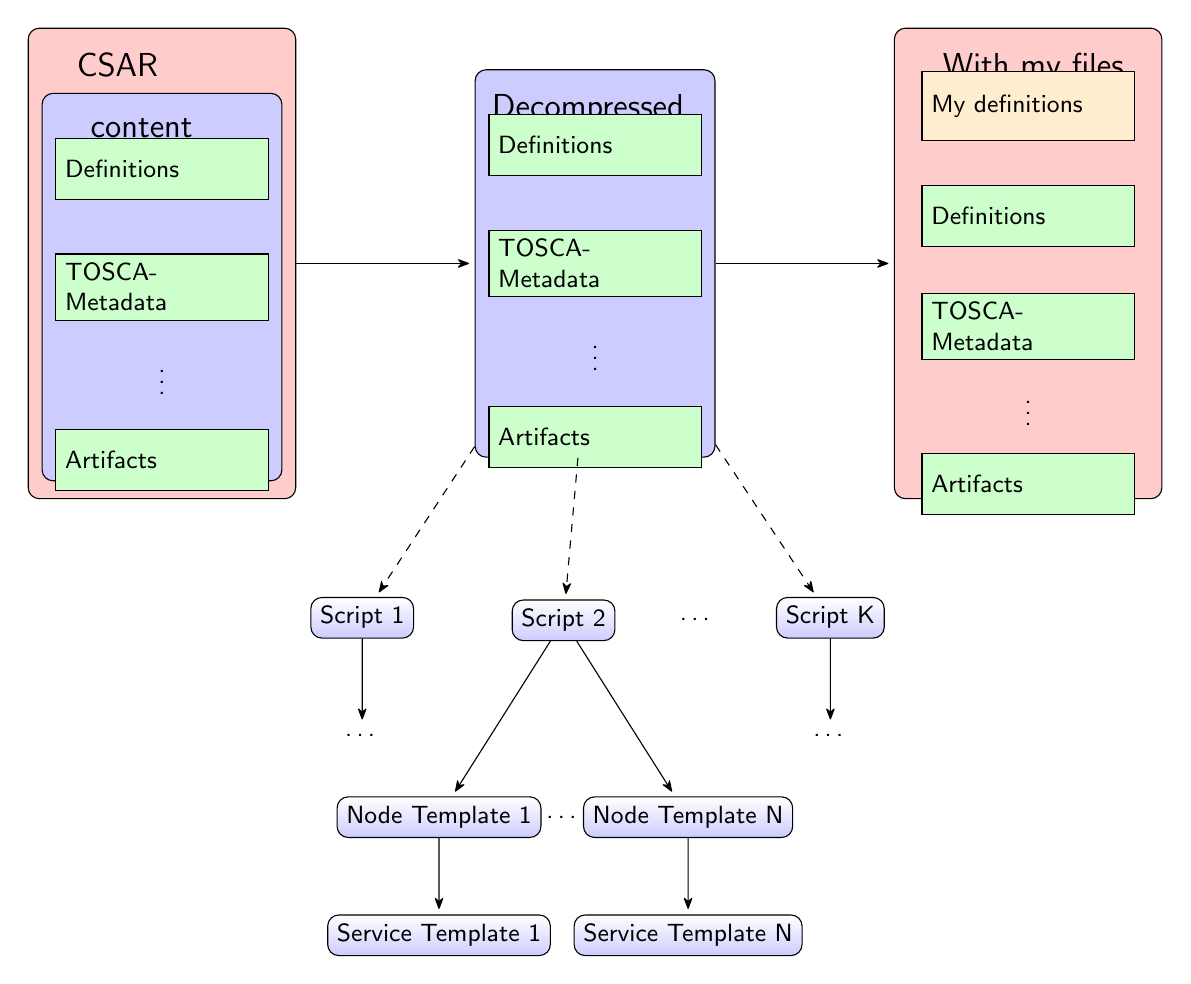
\begin{tikzpicture}[sibling distance=9em,->,>={Stealth[round,sep]},shorten >=1pt,auto,node distance=25mm]


\node (csar_frame) [frame] {};
\node [xshift=+5mm, yshift=-2mm, below right] at (csar_frame.north west) {\large CSAR};

\node (csar_content) at ( [yshift=-3mm]csar_frame) [csar_content] {};
\node [xshift=+5mm, yshift=-2mm, below right] at (csar_content.north west) {\large content};

\node (l2pm1) at ([yshift=+15mm]csar_content) [entry] {Definitions\\};
\node (l2pm2) at ([yshift=0mm]csar_content) [entry] {TOSCA-Metadata\\};
\node (l2pmn) at ([yshift=-22mm]csar_content) [entry] {Artifacts\\};
\node at ($(l2pm2)!.5!(l2pmn)$) {\vdots};
    
\node [right of=csar_frame, xshift=30mm](dc_frame) [csar_content] {};
\node [xshift=+1mm, yshift=-2mm, below right] at (dc_frame.north west) {\large Decompressed};
\draw [->] (csar_frame) -- (dc_frame);
\node (2pm1) at ([yshift=+15mm]dc_frame) [entry] {Definitions\\};
\node (2pm2) at ([yshift=0mm]dc_frame) [entry] {TOSCA-Metadata\\};
\node (2pmn) at ([yshift=-22mm]dc_frame) [entry] {Artifacts\\};
\node at ($(2pm2)!.5!(2pmn)$) {\vdots};

\node [right of=dc_frame, xshift=30mm](my_frame) [frame] {};
\node [xshift=+5mm, yshift=-2mm, below right] at (my_frame.north west) {\large With my files};
\draw [->] (dc_frame) -- (my_frame);
\node (3pmd) at ([yshift=+20mm]my_frame) [myentry] {My definitions\\};
\node (3pm1) at ([yshift=+6mm]my_frame) [entry] {Definitions\\};
\node (3pm2) at ([yshift=-8mm]my_frame) [entry] {TOSCA-Metadata\\};
\node (3pmn) at ([yshift=-28mm]my_frame) [entry] {Artifacts\\};
\node at ($(3pm2)!.5!(3pmn)$) {\vdots};


\node[below=of dc_frame,main node, node distance=10mm, xshift=-4mm, yshift=+7mm] (11) {Script 2}
child { node[main node, yshift=-10mm]  (n21) {Node Template 1} 
		child { node[main node] (s31) {Service Template 1}}  
}
child { node[main node, yshift=-10mm]  (n22) {Node Template N} 
	child { node[main node] (s32) {Service Template N}}  
};
\draw [dashed,->] (dc_frame) -- (11);
\node[below left=of dc_frame,main node,xshift=+10mm] (12) {Script 1}
child { node  {\ldots} 
};
\draw [dashed,->] (dc_frame) -- (12);
\node[below right=of dc_frame,main node, xshift=-10mm] (13) {Script K}
child { node  {\ldots} 
};
\draw [dashed,->] (dc_frame) -- (13);
\node at ($(11)!.5!(13)$) {\ldots};
\node at ($(n21)!.5!(n22)$) {\ldots};

\end{tikzpicture} 
\caption{Preprocessing: decompression, adding files and generating dependencies} 	\label{fig:preproc}
\end{figure}

\subsection{Language modules} \label{subs:archlm}
Each $language$ $module$ describes a handling of one language and chooses files written in the language.
It also contains a list of supported package manager modules.
Each language module must provide the capability to generate a TOSCA node for a given package and this node must use the same language to install the package.
That means, that a script and definitions for Artifact Templates, a Node Type, and a Node Type Implementation should be created by a language module.\\
As already mentioned above, during $processing$ stage a $language$ $module$ analyzes all files one by one and checks their belonging to the language. 
Any files not belonging to the described language are filtered out.
The remaining files are transferred to the $language$ $module$'s $package$ $manager$ $modules$.
For example, a $bash$ module will pass only files with $".sh"$ extension, which start with the $"\#!/bin/bash"$ line.
An $ansible$ module should have an additional functionality to unpack zip archives, where ansible playbooks can be stored.
Since ansible playbooks don't contain specific header or marker, the single sigh of ansible files is the "$.yml$" extension. 

\subsection{Package manager modules} \label{subs:archpmm}
A $package$ $managers$ $module$ finds external references, resolves them and transmits the package name to the $package$ $handler$, described in the next section.
Figure \ref{fig:lang_ph} illustrates data flow between language modules, package manager modules, and the package handler.\\
To resolve an external reference a package manager module will parse a given file. 
In case of the apt-get module for bash, the module will read a file line-by-line searching for the strings starting by "apt-get install".
Such strings must be commented out and those ends should be divided to separate package names, which will be transferred to the package handler. 
% !TeX spellcheck = en_US
\usetikzlibrary{calc,arrows.meta,positioning}
\tikzset{
    every node/.style={font=\sffamily\small},
    main node/.style={shape=rectangle, rounded corners,
    	draw, align=center,
    	top color=white, bottom color=blue!20},
    data node/.style={shape=rectangle,
    draw, align=center,
    top color=white, bottom color=red!20}
}

\begin{figure}
	\centering
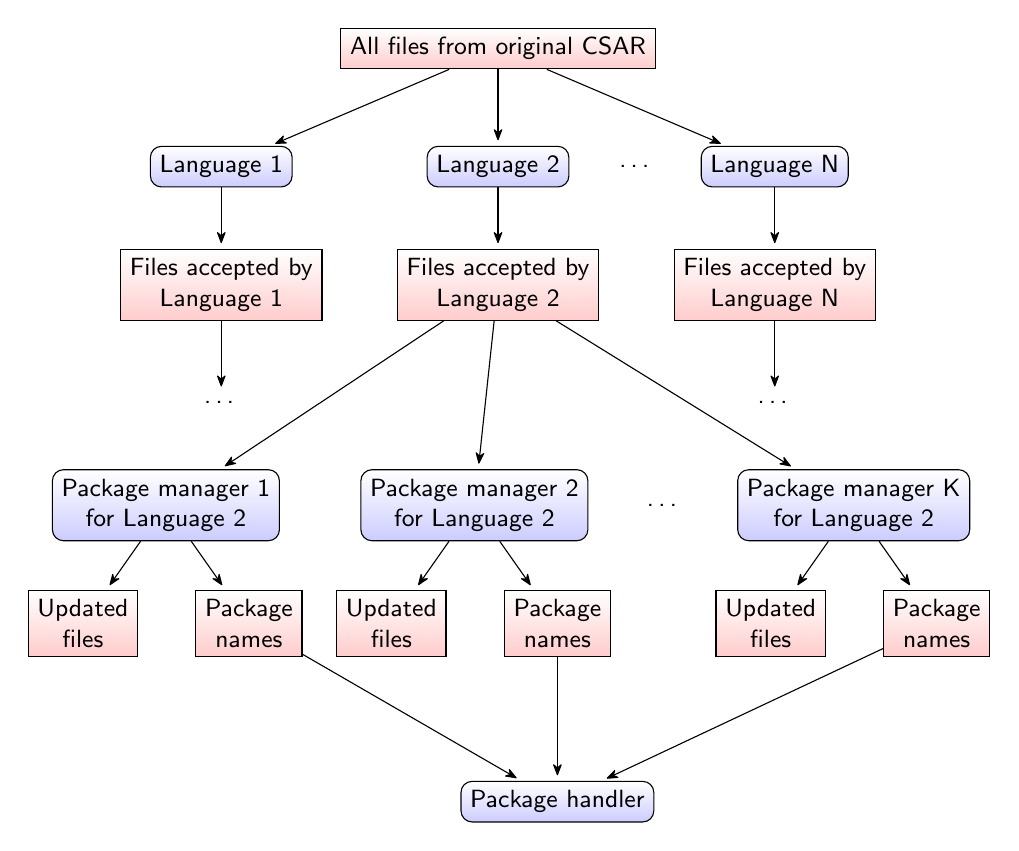
\begin{tikzpicture}[->,>={Stealth[round,sep]},shorten >=1pt,auto,level 1/.style={sibling distance=10em,node distance=25mm},
level 2/.style={sibling distance=8em,node distance=30mm},
level 3/.style={sibling distance=12em,node distance=30mm},
level 4/.style={sibling distance=6em,node distance=25mm},
level 5/.style={sibling distance=8em,node distance=25mm},
level 6/.style={sibling distance=8em,node distance=25mm}]
    \node[data node] (1)  {All files from original CSAR}
    child { node[main node](2) {Language 1} 
    	child { node[data node](21) {Files accepted by\\ Language 1} 
    		child { node {\ldots}}}}
	child { node[main node] (3) {Language 2}
		child { node[data node](31) {Files accepted by\\ Language 2} 
			child { node[main node, yshift=-13mm](32) {Package manager 1\\for Language 2} 
				child { node[data node](36) {Updated\\ files}}
				child { node[data node](37) {Package\\ names}}}
			child { node[main node, yshift=-13mm, xshift=-3mm](33) {Package manager 2\\for Language 2}
				child { node[data node](34) {Updated\\ files}}
				child { node[data node](35) {Package\\ names}}}
			child { node[main node, yshift=-13mm, xshift=+3mm](34) {Package manager K\\for Language 2}
				child { node[data node](38) {Updated\\ files}}
				child { node[data node](39) {Package\\ names}}}
			}
		}
    child { node[main node] (4) {Language N}
    	child { node[data node](41) {Files accepted by\\ Language N} 
    		child { node {\ldots}}}}
	;

	\node [main node,below, yshift=-20mm] at (35) (ph) {Package handler};
    \node at ($(3)!.5!(4)$) {\ldots};
    \node at ($(33)!.5!(34)$) {\ldots};
    \draw [->] (35) --(ph);
    \draw [->] (37) --(ph);
    \draw [->] (39) --(ph);
    
\end{tikzpicture} 
\caption{Data flow scheme between language modules, package manager modules and package handler.} 	\label{fig:lang_ph}
\end{figure}

\subsection{Package Handler} \label{subs:archph}
The $package$ $handler$ becomes a package name, downloads an installation data for an architecture specified by the CSAR handler, transfers the package name to the $topology$ $handler$ and recursively repeats the actions for all depended packages. 
To download an installation data the command "apt-get download \textbf{package}" can be used. 
The architecture can be specified by a ":$architecture$" suffix, for example a "package:$arm$" mean the package of the $arm$ architecture.
The list of dependencies will be obtained using the "apt-cache depends \textbf{package}" command. 
The output of such command should be parsed in order to extract names of depended packages.
Of course in case of fault during a download of a package, an user interface should be provided, to find a solution.
That can be: retry the download, ignore the package, rename the package, or even break the framework's execution.

\subsection{Topology Handler} \label{subs:archtop}
This element should handle the TOSCA topology and has two main tasks: analyze the TOSCA topology during the preprocessing stage to create internal dependencies tries and use those tries to create TOSCA definitions for Node Templates and Relationship Templates in right places for packages provided by the package handler.
The analyze of the TOSCA topology was described in the section \ref{subs:analyse} and the defining of Node Templates and Relationship Templates in the section \ref{subs:repres}.
%$Topology$ $handler$ adds a package to the topology. 
%This includes adding new files and updating existing files. 
%Necessary steps were described in section \ref{subs:repres}.